%\documentclass[12pt,preprint]{aastex}

\documentclass[12pt,manuscript,authoryear]{aastex}

\usepackage{graphicx}

\begin{document}

\title{Migration of Gas Giant Planets in Gravitationally Unstable Disks}
  
\author{{\it Short Title: Gas Giant Migration ~~~~Article Type: Journal}}

\author{Scott Michael}
\affil{Department of Astronomy, Indiana University, Bloomington, IN 47405}
\email{scamicha@astro.indiana.edu}

\and

\author{Richard H. Durisen}
\affil{Department of Astronomy, Indiana University, Bloomington, IN 47405}
\email{durisen@astro.indiana.edu}

\and 

\author{Aaron C. Boley}
\affil{Department of Astronomy; University of Florida,
211 Bryant Space Science Center,
PO Box 112055, Gainesville, FL 32611}
\email{aaron.boley@gmail.com}

\begin{abstract}

Characterization of migration in gravitationally unstable disks is necessary to understand the fate of protoplanets formed by disk instability. As part of a larger study, we are using a 3D radiative hydrodynamics code to investigate how an embedded gas giant planet interacts with a gas disk that is massive enough to experience gravitational instabilities (GIs). This Letter presents preliminary results from simulations with a Jupiter-mass planet placed in orbit at 25 AU within a 0.13 $M_{\odot}$ disk. The disk spans 5 to 40 AU around a 1 $M_{\odot}$ star and is initially only marginally stable. In one simulation, the planet is inserted prior to the initial eruption of GIs; in another, it is inserted only after the disk has settled into a quasi-steady GI-active state, where heating by GIs roughly balances radiative cooling. When the planet is present from the beginning, its own wake stimulates growth of a particular global mode with which it strongly interacts, and the planet plunges inward six AU in about 10$^3$ years. In both cases, there are times when the planet's radial motion is slow and random. At other times, when the planet interacts with a strong spiral mode near the mode's corotation radius, migration both inward and outward can be relatively rapid, covering several AUs over hundreds of years. {\bf See note in Latex file.}
%The assertion in the preceding sentence needs to be verified by analyzing both runs in more detail -- Am(t), periodograms, images zoomed in on the planet to check for arms. The migration is observed; it is the relationship to mode interactions that needs to be checked.
Planet orbit eccentricity tends to fluctuate rapidly and ranges between about 0.02 to 0.1.
\end{abstract}

\keywords{hydrodynamics --- instabilities --- planet-disk interactions --- planets and satellites: formation --- protoplanetary disks}

\label{firstpage}

\section{Introduction}

{\bf See note in Latex file.} 
%Scott: File in some references you know now. Aaron: Suggestions on references?
Migration of gas giant planets due to interactions with a circumstellar gas disk probably plays a major role in defining the architecture of planetary systems (e.g., ???). Work on migration (see review by ???  Balbus \& Terquem or Papaloizou ???) has included gravitational interaction of planets with both laminar and turbulent disks. However,  the self-gravity of the gas disk has usually been ignored, and the effects of radiative cooling and a detailed equation of state (EOS) have only recently been included (Paardekooper ???). Boss (2004 ???) and Mayer et al. (2004) examined radial migration of planet-mass fragments in gravitationally unstable disks, but their disks were violently disrupted by fragmentation under conditions (radii $<$ 40 AU, disk-to-star mass ratios $M_d/M_s \sim 0.1$, and stellar mass $M_s \sim 1\;M_{\odot}$) where this probably should not realistically have happened (Rafikov 2005, 2007; Boley et al. 2006, 2007b; Boley \& Durisen 2008; Forgan et al. 2009; Cai et al. 2010). More recently, fragmentation into clumps with gas giant or brown dwarf masses has been documented in disks that are relatively massive ($M_d/M_s \sim$ a few tenths) and spatially extended (outer radii $>$ 100 AU) (Krumholz et al. 2007; Stamatellos \& Whitworth 2007, 2009, Boley 2009; Hayfield et al. 2010), where fragmentation is expected from semi-analytic arguments (e.g., Clarke ???, Rafikov 2009, Dobson-Robinson et al. 2009). The fate of the clumps depends in part on their radial migration, which is a chaotic and messy affair in a fragmenting disk (e.g., Boley 2009, Boley et al. 2010, Vorobyov \& Basu 2010; Boley \& Durisen 2010). The occurrence of gravitational instabilities (GIs) may be episodic (Vorobyov \& Basu 2005, 2006). Clumps that survive and contract to the dimensions of young planets can later find themselves in a disk that erupts again into GI activity. As the star/disk system evolves, such a protoplanet may end up in a region of a GI-active disk where fragmentation does not occur.

To improve our understanding of how planets migrate in GI-active disks that are not fragmenting, we have begun a systematic study, using numerical 3D radiative hydrodynamics, where we investigate the effects on both the disk and the planet of inserting a planet-mass object into disks susceptible to GIs. Using techniques deployed in earlier research by our group (Pickett et al. 2003; Mej\'ia et al. 2005; Cai et al. 2006, 2008; Boley et al 2006, 2007b), we can identify the dominant spiral waves in a simulation and analyze how the waves interact with the planet's motion. Our goal is to determine both the effect of giant planets on GIs and the effect of GIs on planet migration. Because GIs are sensitive to radiative physics, we use a well-tested radiative scheme (Boley et al. 2007b) and realistic opacities (D'Alessio et al. 2001).  

Section 2 below presents our numerical methods and initial conditions.  We describe the simulation results in Section 3, and discussion them in Section 4.  

\section{Computational Methodology}

\subsection{3-D Radiative Hydrodynamics}

{\bf See note in Latex file.}
%Scott and Aaron: Verify that everything I say here is correct.
The CHYMERA (Computational HYdrodynamics with MultiplE Radiation Algorithms) code (Boley et al. 2007b) is a second-order, explicit, Eulerian scheme on a 3D cylindrical grid. The code uses a realistic equation of state for H$_2$ (Boley et al. 2007a) and integrates an energy equation that includes $PdV$ work, net heating or cooling due to radiative flux divergence, and heating by artificial bulk viscosity. Calculations are done on a uniform cylindrical grid with reflection symmetry about the disk midplane and a resolution ($\varpi$,$\phi$,z) = (512,512,64). The $z$-axis is the rotation axis of the disk. The large number of azimuthal zones is necessary to resolve the planet's Hill sphere and the planet's wake. These simulations utilize the radiative cooling scheme developed and tested in Boley et al. (2007b), where the optically thick monochromatic flux in the $\varpi$ and $\phi$-directions is computed by flux-limited radiative diffusion and where the radiative transport of energy in the $z$-direction is solved using a one-ray discrete ordinate method in both optically thin and thick regions. Although the central star remains fixed at the grid center, we account for acceleration of the reference frame by the planet and by the disk via indirect potentials, as in Michael \& Durisen (2010), and, overall, the planet integration is done using methods similar to those in Nelson et al. (2000). The Rosseland mean and Planck mean opacities and molecular weights in our simulations are the same as those in Boley et al. (2006, 2007b), except that we correct the D'Alessio et al. (2001) gas mean molecular weight to $\mu$ = 2.39.

\subsection{Initial Model and Simulation Conditions}

{\bf See note in Latex file.}
%Scott: Verify the accuracy of all this.

The model disk, based on an equlibrium model in Pickett et al. (2003), orbits a 1 $M_{\odot}$ star and has a mass $M_d = 0.13 M_{\odot}$, inner and outer radii at 5 and 40 AU, and an initial surface density distribution $\Sigma \sim \varpi^{-1}$. The time unit of one ORP (= outer rotation period) is defined as the rotation period of the initial disk at $\varpi \approx$ 32 AU, or about 250 yr. The disk is initially located between radial grid zones ??? 30 ??? and 240 and is close to isentropic, which results in a Toomre-$Q$ distribution with a marginally unstable (see Durisen et al. 2007) minimum value of ??? at radial grid zone ??? (??? AU). The computational grid extends radially to 512 zones to accommodate expansion of the outer disk once GIs become nonlinear. There is an inner cylindrical hole in the grid with a radius of 13 radial zones. To seed nonaxisymmetry, the density is given an initial ??? \% random cell-to-cell perturbation.

This Letter presents three simulations. The first, which we call the fiducial run, goes from time $t = 0$ to ??? 20 ??? ORP without a planet. In the second simulation, which we call the $t = 0$ planet run, a one Jupiter-mass ($M_J$) planet with a roughly circular midplane orbit is included in the initial $t = 0$ ORP equilibrium disk at 25 AU. In the third simulation, which we call the $t = 10$ planet run, a 1 $M_J$ planet with a similar orbit is inserted into the fiducial run at $t = 10$ ORP. These three simulations are part of a much larger suite, to be described elsewhere, in which the planet mass and starting locations are varied. We estimate crude semi-major axes $a$ and eccentricities $e$ from the planet's $\varpi(t)$ by finding at the maximum and minimum radii, $\varpi_{\rm max}$ and $\varpi_{\rm min}$, over each interval that the planet's $\phi$ changes by 2$\pi$ (one ``orbit'') and then using $a = (\varpi_{\rm max}+\varpi_{\rm min})/2$ and $e = (\varpi_{\rm max}-\varpi_{\rm min})/(\varpi_{\rm max}+\varpi_{\rm min})$. These orbital elements are only intended to be indicative; there are strong orbit to orbit variations in these $a$ and $e$.

\section{Results}

{\it The Fiducial Run.} As in Mej\'ia et al (2005), the fiducial run exhibits four distinct phases: initial {\sl axisymmetric cooling}, the onset of GIs in a well-defined {\sl burst}, a {\sl transition}, and the {\sl asymptotic} establishment of quasi-steady chaotic GI-activity with an overall balance of heating and cooling. There is no fragmentation because this disk has a long cooling time (see Gammie 2001; Boley et al. 2006, 2007b).

%Scott: A number of things in this paragraph need to verified by further analysis.
{\it The $t = 0$ Planet Run.} {\bf See note in Latex file.} Figure \ref{fig:Am} shows that inclusion of even this modest mass planet ($0.8 \%$ of $M_d$) has a dramatic effect on the burst phase. Without a planet, when all modes grow from imposed noise, it takes 4 ORPs for coherent spiral modes to organize and grow to nonlinear amplitude. The growth is centered near the $Q$-minimum at ??? AU. Modes of cos($m\phi$) symmetry with $m =$ 5 and 6 dominate. An $m = 3$ (three-armed) spiral also grows somewhat more slowly, but lags the other modes in time. In the $t = 0$ planet run, the planet develops an organized wake within about an ORP in which $m = 3$ is a dominant component ($\sim 5$ \% global density perturbation). This nonlinear seeding causes $m = 3$ to dominates the GI burst, which also occurs $\sim$ 2 ORPs earlier. Because of our initial placement of the planet inside but close to the $Q$-minimum, the corotation radius (CR) of the $m = 3$ mode is fairly close to that of the planet's orbit period. When the triggered $m = 3$ mode becomes strongly nonlinear at about 3 ORP, planet migration is significantly affected. Figure \ref{fig:a} shows the evolution of the planet's radial position. From 0 to 2.5 ORP, the planet is torqued primarily by its own wake and migrates inward. Beginning at 3 ORP, when the $m = 3$ mode has grown significantly and the planet is lagging one of its arms in azimuth, the planet gains angular momentum and moves outward. At about $t =$ 4 ORP, as the planet overtakes the arm, the sign of the net torque reverses and the planet plunges from 23 to 17 AU in about 4 ORP (10$^3$ yr). During this time, the planet and mode seem to interact strongly enough that the planet essentially surfs along the arm, maintaining a location within the arm as it plunges. After $t =$ 8 ORP, the main burst is over, and the disk transitions into its asymptotic state, where modes of many $m$-values are comparably strong. The planet's radial migration apparently stalls at about 16 to 17 AU. From an analysis of periodicities present in the gas disk between 8 and 12 ORP, the planet lies a few AU inside the inner Lindblad resonance of a strong $m = 2$ mode with CR at ??? AU in the GI-active disk. 

%Scott: Even more work is needed to verify what is said here. Some of what I wrote is pure speculation and needs to be checked.
{\it The $t = 10$ Planet Run.} {\bf See note in Latex file.} The motion of the planet in this case is more difficult to interpret. We see intervals of fairly rapid inward or outward migration over several orbits, as well as times when radial migration appears to stall. Between $t = 15$ and 19 ORP, the pattern of outward migration for 2 ORP followed by an inward plunge over the next 2 ORP resembles the behavior in the $t = 0$ planet run during the burst, but, in this case, there is no distinct phase of GI activity. Animations of the simulation show there is a complex interaction between the planet, its spiral wake, and the global spiral arms caused by the instabilities. Analysis of images and periodicities suggests that, between 15 and 19 ORP, the planet may have passed through an arm of an $m =$ ??? pattern with CR at ??? AU. It is possible that the planet actually stimulated this particular mode, in manner similar to what occurred in the $t = 0$ planet run, because this $m =$ ??? periodicity is absent over the same time interval in the fiducial run.

{\it Eccentiricity.} Figure \ref{fig:e} shows the evolution of $e$ in the planet simulations. In both cases, the planets were inserted with an approximate circular velocity computed by adding the interior disk mass to the stellar point mass. The presence of GI activity in the $t = 10$ planet run immediately increases $e$ to $\sim 0.08$. In the $t = 0$ planet run, the modest initial $e$ decreases, as it should (ref ???), during the 1.5 ORP when it is migrating only due to its own wake. However, once there are strong nonlinear interactions with GI modes, $e$ jumps upward. In both runs, it appears that interaction with well-established GI activity leads to eccentricities between 0.02 and 0.1 that vary in a chaotic way between these extremes on orbit period time scales. 

{\it Migration Relative to the Disk.} The disk surface density distribution does not vary much in the asymptotic phase, so radial motion of the planet in the $t = 10$ planet run also represents radial migration relative to the gas. During the burst (e.g., Boley et al. 2006), the surface density of the disk changes dramatically. To verify that the planet is really migrating relative to the background gas disk in the $t = 0$ run, we have compared the evolution of the planet's radial position $\varpi_p(t)$ with the mass inside that radius, expressed in terms of $m_{\rm cyl}$, the fraction of the disk mass interior to the planet. Between $t = 3.52$ and $3.89$ ORP, when $\varpi_p$ increases modestly, $m_{\rm cyl}$ increases from about 0.50 to 0.53; between 3.89 and 8.47 ORP, when $\varpi_p$ decreases dramatically, $m_{\rm cyl}$ also decreases dramatically from 0.53 to 0.30. So, the planet is migrating significantly with respect to the disk mass even while the inner part of the gas disk is moving inward during the burst. For a comparison measure of the magnitude of the gas motion, $m_{\rm cyl}$ at 23 AU increases from 0.50 to 0.60 from $t =$ 3.89 to 8.47 ORP, corresponding to an gas disk inflow rate of $\sim 10^{-5} M_{\odot}/{\rm yr}$.

\section{Discussion}

{\bf See notes in Latex file.}
%Scott and Aaron: This section needs a lot of help.

Check against estimated type I migration without GIs. 
%Aaron: Can you do this?} 
Figure \ref{fig:a} suggests that the overall radial drift is not too different, but it is definitely not monotonic and can stall. Further work is needed to determine how long the stalls last.

Even in non-self-gravitating disks, the presence of discrete radial structure is known to cause instabilities (Li and Lovelace articles abound 2000, 2001). Meschiari \& Laughlin (2008) recently demonstrated that a gap, presumably opened by an embedded planet, can cause global modes to become unstable in self-gravitating disks that are otherwise stable against the development of GIs. Here we are dealing with a planet that is not massive enough to open a gap, but its gravitational interaction with the disk also has a strong effect on the growth and onset of GIs.

Discrete mode interactions with the planet seem important -- Wind up and pitch? Surfing?

Stalling at LRs?
In both cases it is interesting to note that inward migration halts near 17 AU (coincidence???) ; this may be an artifact of the length of the simulations, clearly both simulations should be carried further. This radius is interesting because it is the location of the Inner Linblad Resonance (ILR) for the strong m = 2 mode present in the baseline simulation. Inside the ILR the mode can not effectively transfer angular momentum between the disk and the planet. Further work is necessary to adequately analyze the Fourier modes and their periodicities in the simulations with planets, but this gives a strong preliminary indication that the GI activity is driving the migration. Furthermore, where GIs are inactive planet migration is stalled, even Type I migration may be ineffective due to interference from the GIs at the planet�s OLR.

Not a simple random walk for this mass and this disk. Need to know dependence on planet mass and initial location.

Magnitude of $e$ is roughly consistent with $c_s/v_K$ and low Mach number spirals.

The inclusion of a 1$M_J$ mass in the equilibrium disk initiates GIs and dramatically effects the character of the GIs. GIs can cause both inward and outward planet migration and can cause rapid migration in the burst phase.
GIs can have a strong effect on the orbital eccentricity of the included planet.

\section{Acknowledgments}

The authors would like to thank F.C. Adams and J.C.B. Papaloizou for useful encouragement in this project. The research was conducted with the support of NASA grants from the Origins of Solar Systems  Program (NNG05GN11G and NNX08AK36G). {\bf Scott: Add necessary UITS and Teragrid acknowledgments.}

\begin{thebibliography}{99}

\bibitem[\protect\citeauthoryear{Boley}{2009}]{boley09} 
Boley,  A.C. 2009, ApJ, 695, L53 

\bibitem[\protect\citeauthoryear{Boley \& Durisen}{2006}]{bd06} Boley, A.C., Durisen, R.H. 2006, ApJ, 641, 534

\bibitem[\protect\citeauthoryear{Boley \& Durisen}{2008}]{bd08} Boley, A.C., Durisen, R.H. 2008, ApJ, 685, 1193

\bibitem[\protect\citeauthoryear{Boley et al.}{2006}]{boley06} Boley, A.C., 
Mej\'ia, A.C., Durisen, R.H., Cai, K., Pickett, M.K. 2006, ApJ, 651, 517

\bibitem[\protect\citeauthoryear{Boley et al.}{2007}]{boley07} Boley, A.C., 
Durisen, R.H., Nordlund, A., Lord, J. 2007, ApJ, 665, 1254 

\bibitem[\protect\citeauthoryear{Boley et al.}{2009}]{boleyetal09} Boley, A.C., 
Hayfield, T., Mayer, L., Durisen, R.H.  2010, Icarus, in press (arXiv:0909.4543)

\bibitem[\protect\citeauthoryear{Boss}{1984}]{boss84} Boss, A.P. 1984, ApJ, 277, 768

\bibitem[\protect\citeauthoryear{Boss}{1997}]{boss97} Boss, A.P. 1997, Science, 267, 1836

\bibitem[\protect\citeauthoryear{Boss}{1998}]{boss98} Boss, A.P. 1998, ApJ, 503, 923

\bibitem[\protect\citeauthoryear{Boss}{2000}]{boss00} Boss, A.P. 2000, ApJ, 536, L101

\bibitem[\protect\citeauthoryear{Boss}{2001}]{boss01} Boss, A.P. 2001, ApJ, 563, 367

\bibitem[\protect\citeauthoryear{Boss}{2002}]{boss02} Boss, A.P. 2002, ApJ, 576, 462

\bibitem[\protect\citeauthoryear{Boss}{2003}]{boss03} Boss, A.P. 2003, ApJ, 599, 577

\bibitem[\protect\citeauthoryear{Boss}{2004}]{boss04} Boss, A.P. 2004, ApJ, 610, 456

\bibitem[\protect\citeauthoryear{Boss}{2005}]{boss05} Boss, A.P. 2005, ApJ, 629, 535

\bibitem[\protect\citeauthoryear{Boss}{2007}]{boss07} Boss, A.P. 2007, ApJ, 661, L73

\bibitem[\protect\citeauthoryear{Boss}{2009}]{boss09} Boss, A.P. 2009, ApJ, 694, 107

\bibitem[\protect\citeauthoryear{Cai et al.}{2006}]{cai06} Cai, K., Durisen, R.H., Michael, S., Boley, A.C., Mej\'ia, A.C., Pickett, M.K., D'Alessio, P. 2006, ApJ, L149

\bibitem[\protect\citeauthoryear{Cai et al.}{2008}]{cai08} Cai, K., Durisen, R.H., Boley, A.C., Pickett, M.K., Mej\'ia, A.C. 2008, ApJ, 673, 1138

\bibitem[\protect\citeauthoryear{Clarke}{2009}]{clarke09} 
Clarke, C.J. 2009, MNRAS, 396, 1066

\bibitem[\protect\citeauthoryear{D'Alessio et al.}{2001}]{dalessio01} D'Alessio, P., Calvet, N., Hartmann, L. 2001, ApJ, 553, 321

\bibitem[\protect\citeauthoryear{Dodson-Robinson et al.}{2009}]{dodson09}
Dodson-Robinson, S. E., Veras, D., Ford, E. B., Beichman, C. A. 2009, ApJ, 707, 79

%\bibitem[\protect\citeauthoryear{Durisen, Mej\'ia, \& Pickett}
%{Durisen et al.}{2003}]{durisen03} Durisen, R.H., Mej\'ia, A.C., 

\bibitem[\protect\citeauthoryear{Durisen et al.}{2007}]{durisen07} Durisen R.H., Boss, A.P., Mayer, L., Nelson, A.F., Quinn, T., Rice, W.K.M. 2007, in: Protostars and Planets V, ed. B. Reipurth, D. Jewitt, \& K. Keil (Tucson:  Univ. of Arizona Press), 607

\bibitem[\protect\citeauthoryear{Durisen et al.}{2008}]{durisen08} 
Durisen R.H., Hartquis, T.W., \& Pickett M.K., Durisen R.H. 2008, ApSpSci., 317, 3 

\bibitem[\protect\citeauthoryear{Forgan et al.}{2009}]{forg09} Forgan, D., Rice, K., Stamatellos, D., Whitworth, A. 2009, MNRAS 394, 882

\bibitem[\protect\citeauthoryear{Gammie}{2001}]{gammie01} Gammie, C.F. 2001, ApJ, 553, 174 

\bibitem[\protect\citeauthoryear{Johnson \& Gammie}{2003}]{johnson03} 
Johnson, B.M., Gammie, C.F. 2003, ApJ, 597, 131 

\bibitem[\protect\citeauthoryear{Haisch et al.}{2001}]{haisch01} 
Haisch, K.E., Jr., Lada, E.A., Lada, C.J. 2001, ApJ, 553, L153

\bibitem[\protect\citeauthoryear{Hayfield et al.}{2010}]{hayfield10}
Hayfield, T., Mayer, L., Wadsley, J., Boley, A. C. 2010, arXiv:1003.2594

\bibitem[\protect\citeauthoryear{Mayer et al.}{2002}]{mayer02} Mayer, L., Quinn, T. Wadsley, J., Stadel, J. 2002, Science, 298, 1756

\bibitem[\protect\citeauthoryear{Mayer et al.}{2004}]{mayer04} Mayer, L., Quinn, T., Wadsley, J., Stadel, J. 2004, ApJ, 609, 1045 

\bibitem[\protect\citeauthoryear{Mayer et al.}{2007}]{mayer07} 
Mayer, L., Lufkin, G., Quinn, T., Wadsley, J. 2007, ApJ, L77 

\bibitem[\protect\citeauthoryear{Mej\'ia et al.}{2005}]{mejia05} Mej\'ia, A.C., Durisen, R.H., Pickett, M.K., Cai, K. 2005, ApJ, 619, 1098 

\bibitem[\protect\citeauthoryear{Nelson}{2006}]{nelson06} Nelson A.F. 2006, MNRAS, 373, 1039

\bibitem[\protect\citeauthoryear{Nelson et al.}{1998}]{nelson98} Nelson, A.F., Benz, W., Adams, F.C., Arnett, D. 1998, ApJ, 502, 342 

\bibitem[\protect\citeauthoryear{Nelson, Benz, Ruzmaikina}{Nelson et al.}{2000}]
{nelson00} Nelson, A.F., Benz, W., Ruzmaikina, T.V. 2000, ApJ, 529, 357 

\bibitem[\protect\citeauthoryear{Pickett et al.}{1998}]{pickett98} Pickett, B.K., Cassen, P., Durisen, R.H., Link, R. 1998, ApJ, 504, 468

\bibitem[\protect\citeauthoryear{Pickett et al.}{2000a}]{pickett00a} Pickett, B.K., Cassen, P., Durisen, R.H., Link, R. 2000, ApJ, 529, 1034

\bibitem[\protect\citeauthoryear{Pickett et al.}{2000b}]{pickett00b} Pickett, B.K., Durisen, R.H., Cassen, P., Durisen, R.H., Mej\'ia, A.C. 2000, ApJ, 540, L95

\bibitem[\protect\citeauthoryear{Pickett et al.}{2003}]{pickett03} Pickett, B.K., Mej\'ia, A.C., Durisen, R.H., Cassen, P., Berry, D.K., Link, R.P. 2003, ApJ, 590, 1060

\bibitem[\protect\citeauthoryear{Pickett \& Durisen}{2007}]{pickett07} 
Pickett, M.K., Durisen, R.H. 2007, ApJ, 654, L155 

\bibitem[\protect\citeauthoryear{Rafikov}{2005}]{rafikov05} 
Rafikov,  R.R. 2005, ApJ, 621, L69 

\bibitem[\protect\citeauthoryear{Rafikov}{2007}]{rafikov07} 
Rafikov,  R.R. 2007, ApJ, 662, 642 

\bibitem[\protect\citeauthoryear{Rafikov}{2009}]{rafikov09} 
Rafikov,  R.R. 2009, ApJ, 704, 281

\bibitem[\protect\citeauthoryear{Rice et al.}{2003}]{rice03} Rice, W.K.M., Armitage, P.J., Bate, M.R., Bonnell, I.A. 2003, MNRAS, 339, 1025

\bibitem[\protect\citeauthoryear{Rice et al.}{2005}]{rice05} Rice, W.K.M., Lodato, G., Armitage, P.J. 2005, MNRAS, 364, L56 

\bibitem[\protect\citeauthoryear{Stamatellos \& Whitworth}{2008}]{stam08} Stamatellous, D., \& Whitworth, A. 2008, A\& A, 480, 879

\bibitem[\protect\citeauthoryear{Stamatellos \& Whitworth}{2009}]{stam09} Stamatellous, D., \& Whitworth, A. 2009, MNRAS, 392, 413

\bibitem[\protect\citeauthoryear{Vorobyov \& Basu}{2010}]{vb10}
Vorobyov, E.I., Basu, S. 2010, ApJ, 714, L133

\bibitem[\protect\citeauthoryear{Zhu et al.}{2009}]{zhu09} Zhu, Z., Hartmann, L., Gammie, C.F.; McKinney, J.C. 2009, ApJ, 701, 620


\end{thebibliography}

\newpage

\begin{figure}[t]
\center
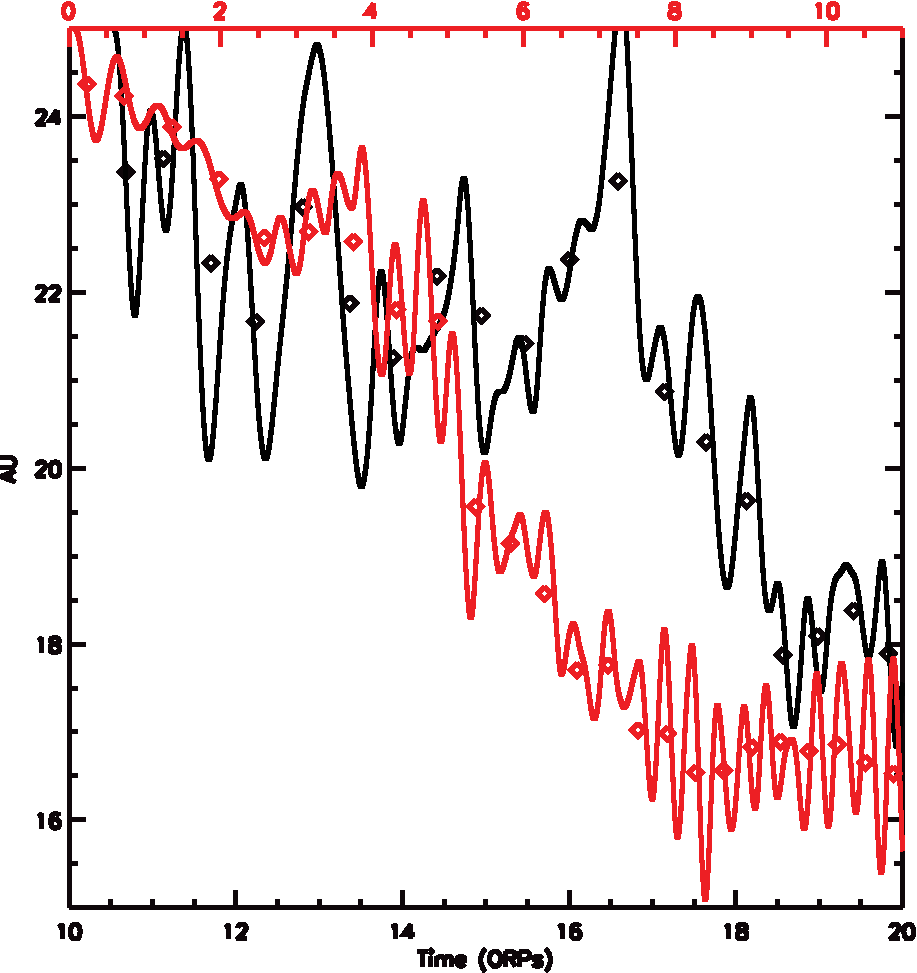
\includegraphics[width=12cm]{../Figures/planeta.pdf}
\caption{Global amplitudes of nonaxisymmetric density perturbations $A_m$ as a function of time for individual cos($m\phi$) perturbations. The formula for computing $A_m$ is equation (15) of Boley et al. (2006). Here the integrals are done only over the disk outside 15 AU to suppress contributions from edge effects in the inner disk. The set of red and black curves correspond to the $t = 0$ and $t = 10$ planet runs, respectively. {\bf The radial migration plot is being used as a placeholder.}}
\label{fig:Am}
\end{figure}

\begin{figure}[t]
\center
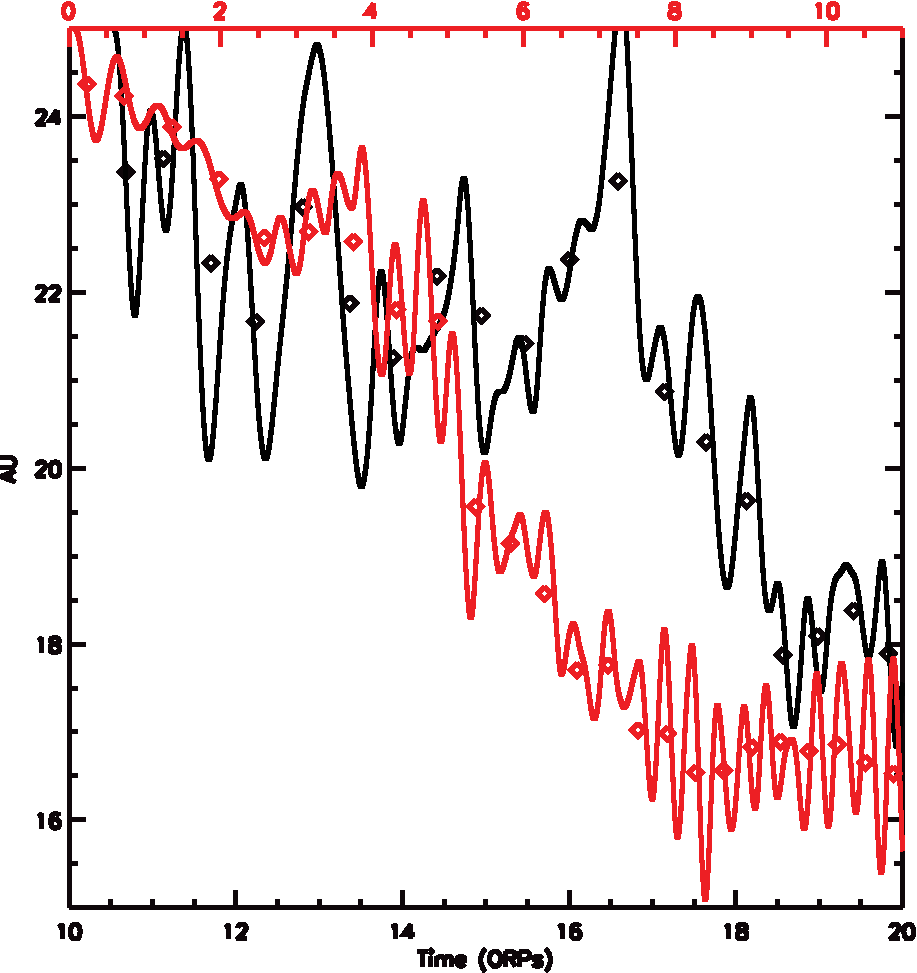
\includegraphics[width=12cm]{../Figures/planeta.pdf}
\caption{Plot of the planet's radial position as a function of time $\varpi_p(t)$ for the two planet simulations. The red and black indicate the curves ($\varpi(t)$), points ($a$), and horizontal scales ($t$) that correspond to the $t = 0$ and $t = 10$ planet runs, respectively. The diamonds are the approximate semi-major axes $a$ computed for each 0 to 2$\phi$ change in azimuth of the planet as explained in the text.}
\label{fig:a}
\end{figure}

\begin{figure}[t]
\center
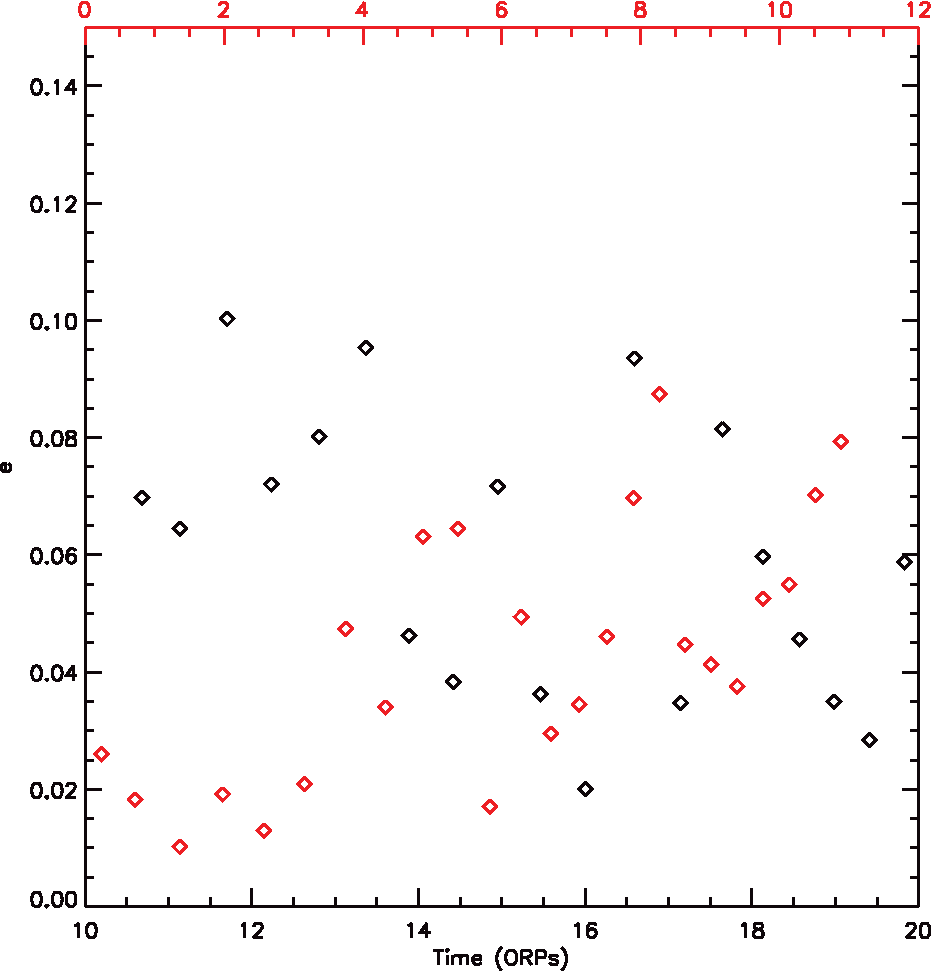
\includegraphics[width=12cm]{../Figures/planete.pdf}
\caption{Plot of the eccentricities $e$, computed for each 0 to 2$\phi$ change in azimuth of the planet as explained in the text, as a function of time. The red and black indicate the points ($e$) and horizontal scales ($t$) that correspond to the $t = 0$ and $t = 10$ planet runs, respectively.}
\label{fig:e}
\end{figure}

%\begin{figure}[t]
%\includegraphics{../Figures/name_of_figure.eps}
%\caption{here's the caption}
%\label{fig:name}
%\end{figure}

\label{lastpage}

\end{document}


